
\section{Method}
\label{sec:method}

\begin{figure} 	
\centering 	
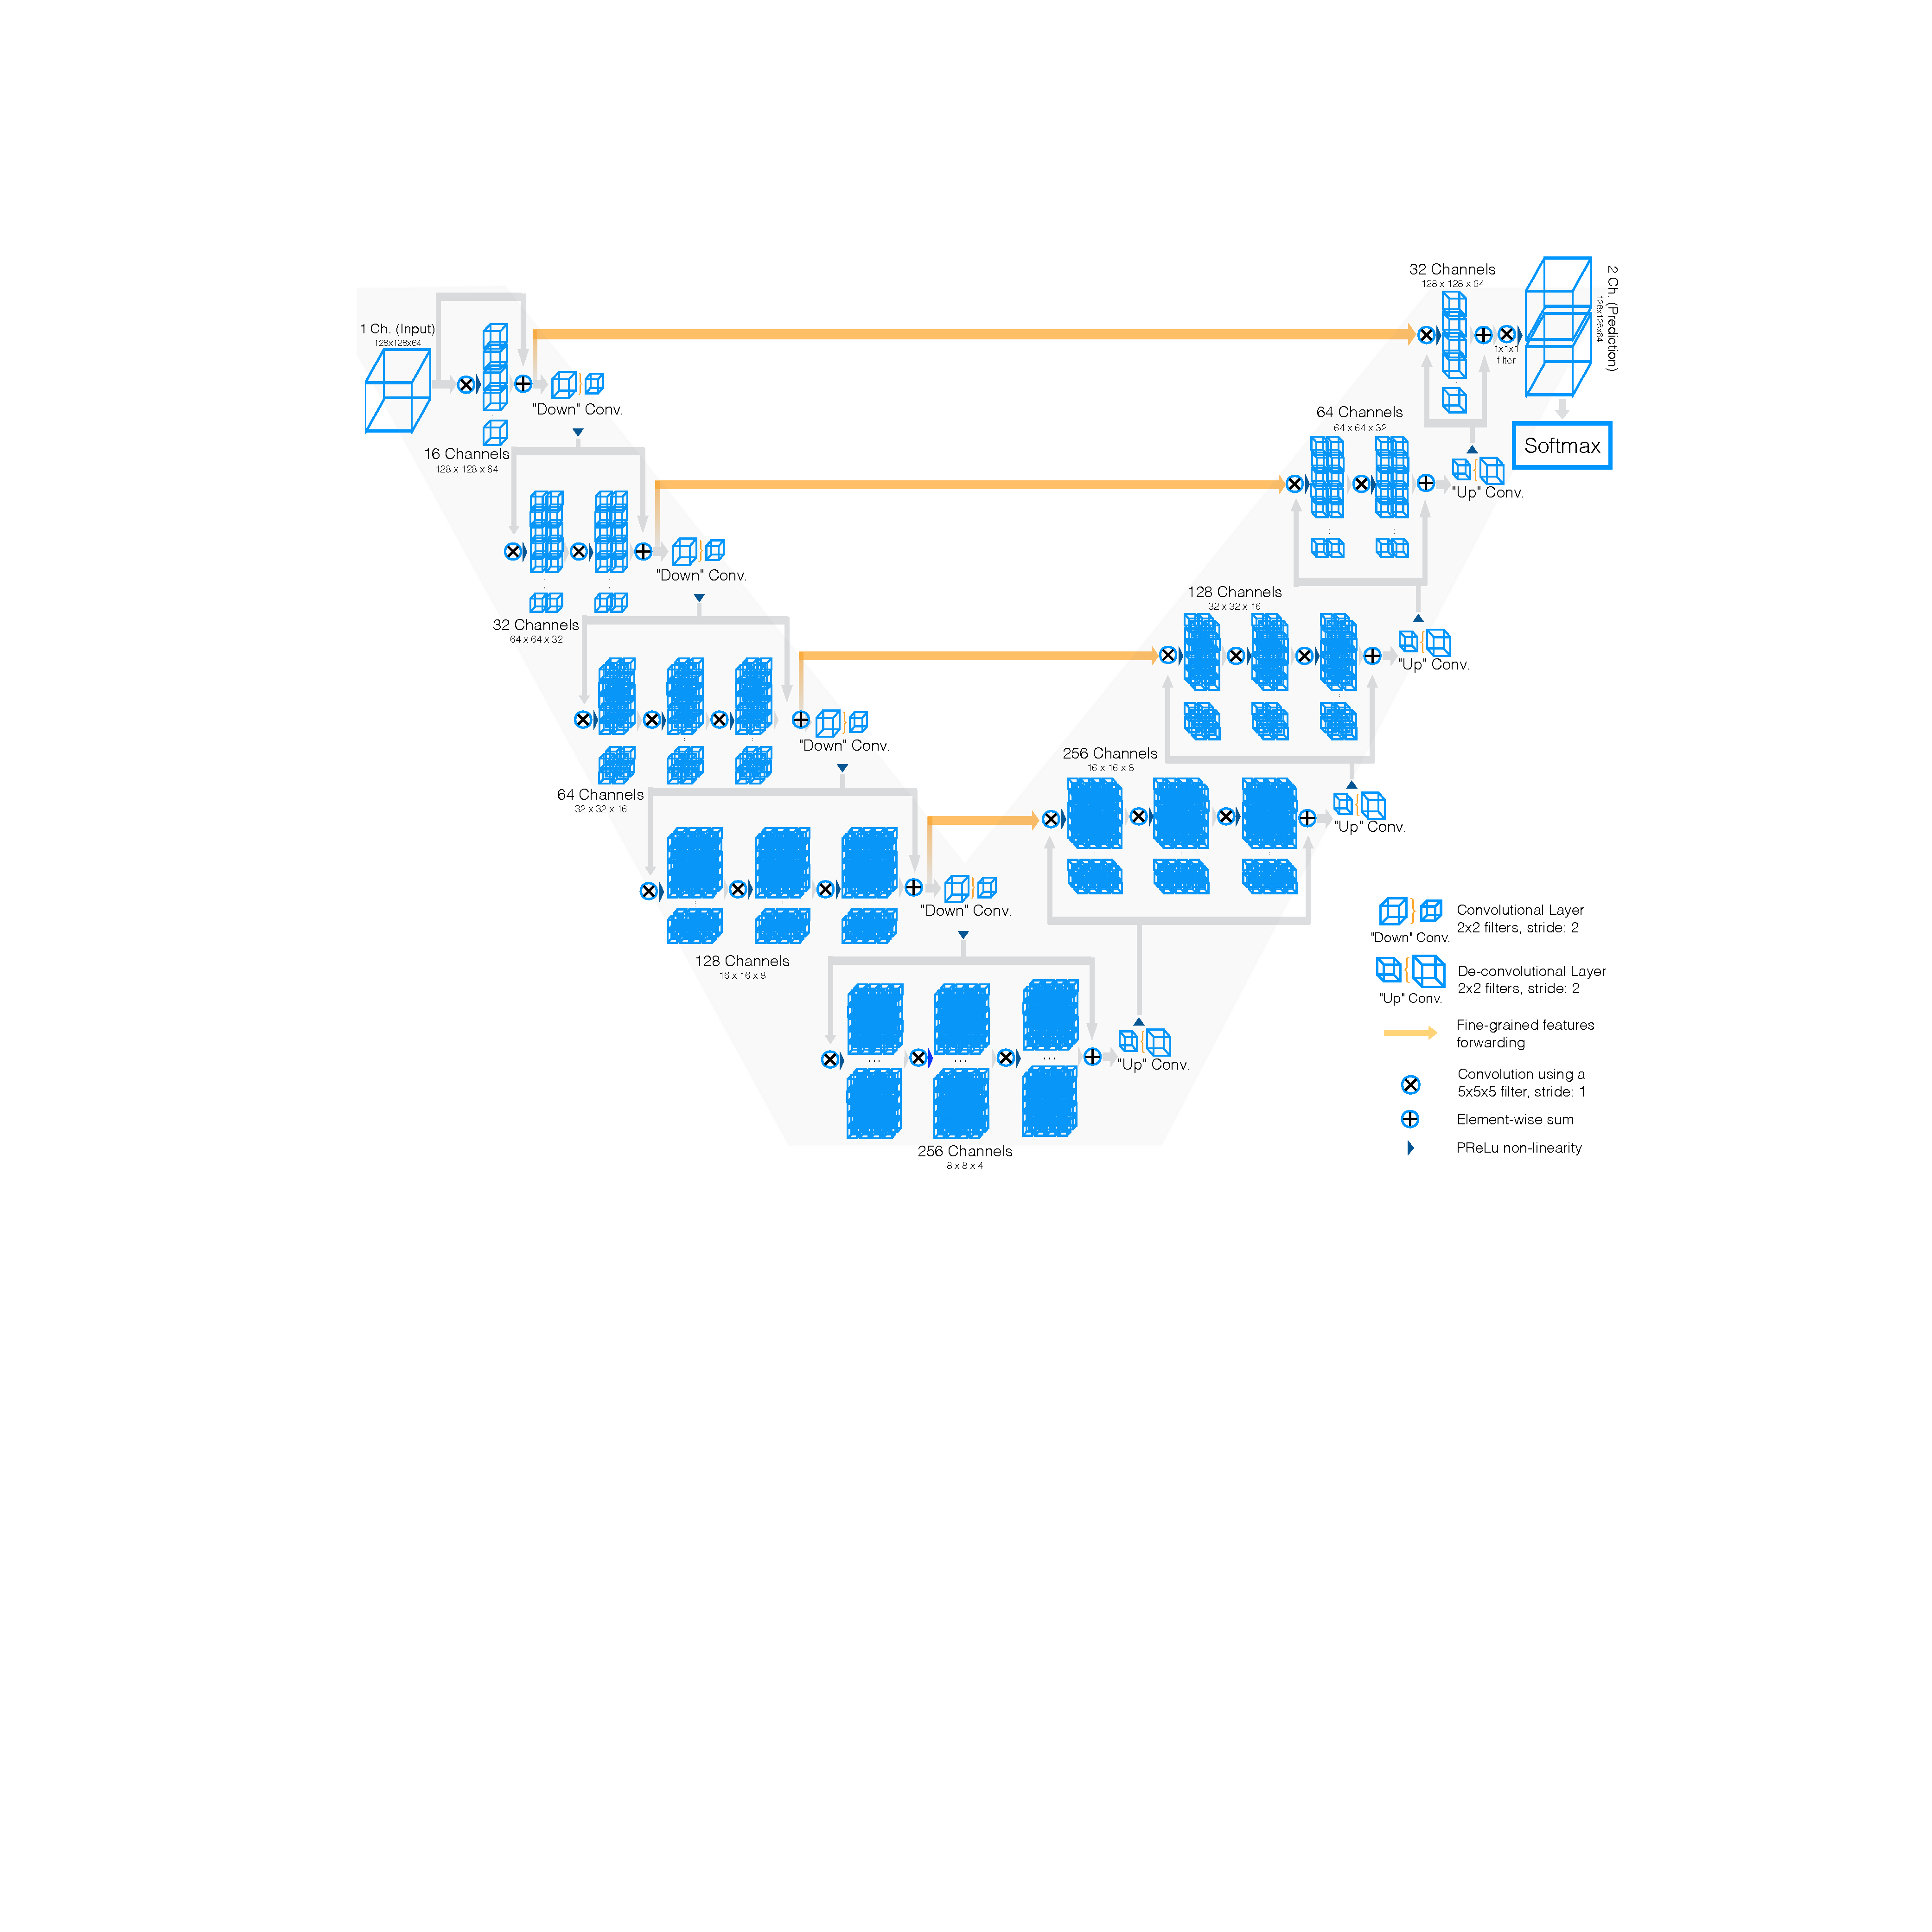
\includegraphics[scale=0.26]{architecture.pdf} 	
\caption{Schematic representation of our network architecture. Our custom implementation of Caffe \cite{jia2014caffe} processes 3D data by performing volumetric convolutions. Best viewed in electronic format.} \label{fig:VnetImage} 
\end{figure}

In Figure \ref{fig:VnetImage} we provide a schematic representation of our convolutional neural network. 
We perform convolutions aiming to both extract features from the data and, at the end of each stage, to reduce its resolution by using appropriate stride. The left part of the network consists of a compression path, while the right part decompresses the signal until its original size is reached. Convolutions are all applied with appropriate padding.

The left side of the network is divided in different stages that operate at different resolutions. Each stage comprises one to three convolutional layers. Similarly to the approach presented in \cite{he2015deep}, we formulate each stage such that it learns a residual function: the input of each stage is (a) used in the convolutional layers and processed through the non-linearities and (b) added to the output of the last convolutional layer of that stage in order to enable learning a residual function. As confirmed by our empirical observations, this architecture ensures convergence in a fraction of the time required by a similar network that does not learn residual functions. 

The convolutions performed in each stage use volumetric kernels having size $5\times5\times5$ voxels.
As the data proceeds through different stages along the compression path, its resolution is reduced. This is performed through convolution with $2\times2\times2$ voxels wide kernels applied with stride $2$ (Figure \ref{fig:updown}). Since the second operation extracts features by considering only non overlapping $2\times2\times2$ volume patches, the size of the resulting feature maps is halved. 
This strategy serves a similar purpose as pooling layers that, motivated by \cite{springenberg2014striving} and other works discouraging the use of max-pooling operations in CNNs, have been replaced in our approach by convolutional ones. Moreover, since the number of feature channels doubles at each stage of the compression path of the V-Net, and due to the formulation of the model as a residual network, we resort to these convolution operations to double the number of feature maps as we reduce their resolution. PReLu non linearities are applied throughout the network.

Replacing pooling operations with convolutional ones results also to networks that, depending on the specific implementation, can have a smaller memory footprint during training, due to the fact that no switches mapping the output of pooling layers back to their inputs are needed for back-propagation, and that can be better understood and analysed \cite{zeiler2014visualizing} by applying only de-convolutions instead of un-pooling operations. 

Downsampling allows us to reduce the size of the signal presented as input and to increase the receptive field of the features being computed in subsequent network layers. Each of the stages of the left part of the network, computes a number of features which is two times higher than the one of the previous layer.

The right portion of the network extracts features and expands the spatial support of the lower resolution feature maps in order to gather and assemble the necessary information to output a two channel volumetric segmentation. The two features maps computed by the very last convolutional layer, having $1\times1\times1$ kernel size and producing outputs of the same size as the input volume, are converted to probabilistic segmentations of the foreground and background regions by applying soft-max voxelwise.
After each stage of the right portion of the CNN, a de-convolution operation is employed in order increase the size of the inputs (Figure \ref{fig:updown}) followed by one to three convolutional layers involving half the number of $5\times5\times5$ kernels employed in the previous layer. Similar to the left part of the network, also in this case we resort to learn residual functions in the convolutional stages.

\begin{figure} 	
\centering 	
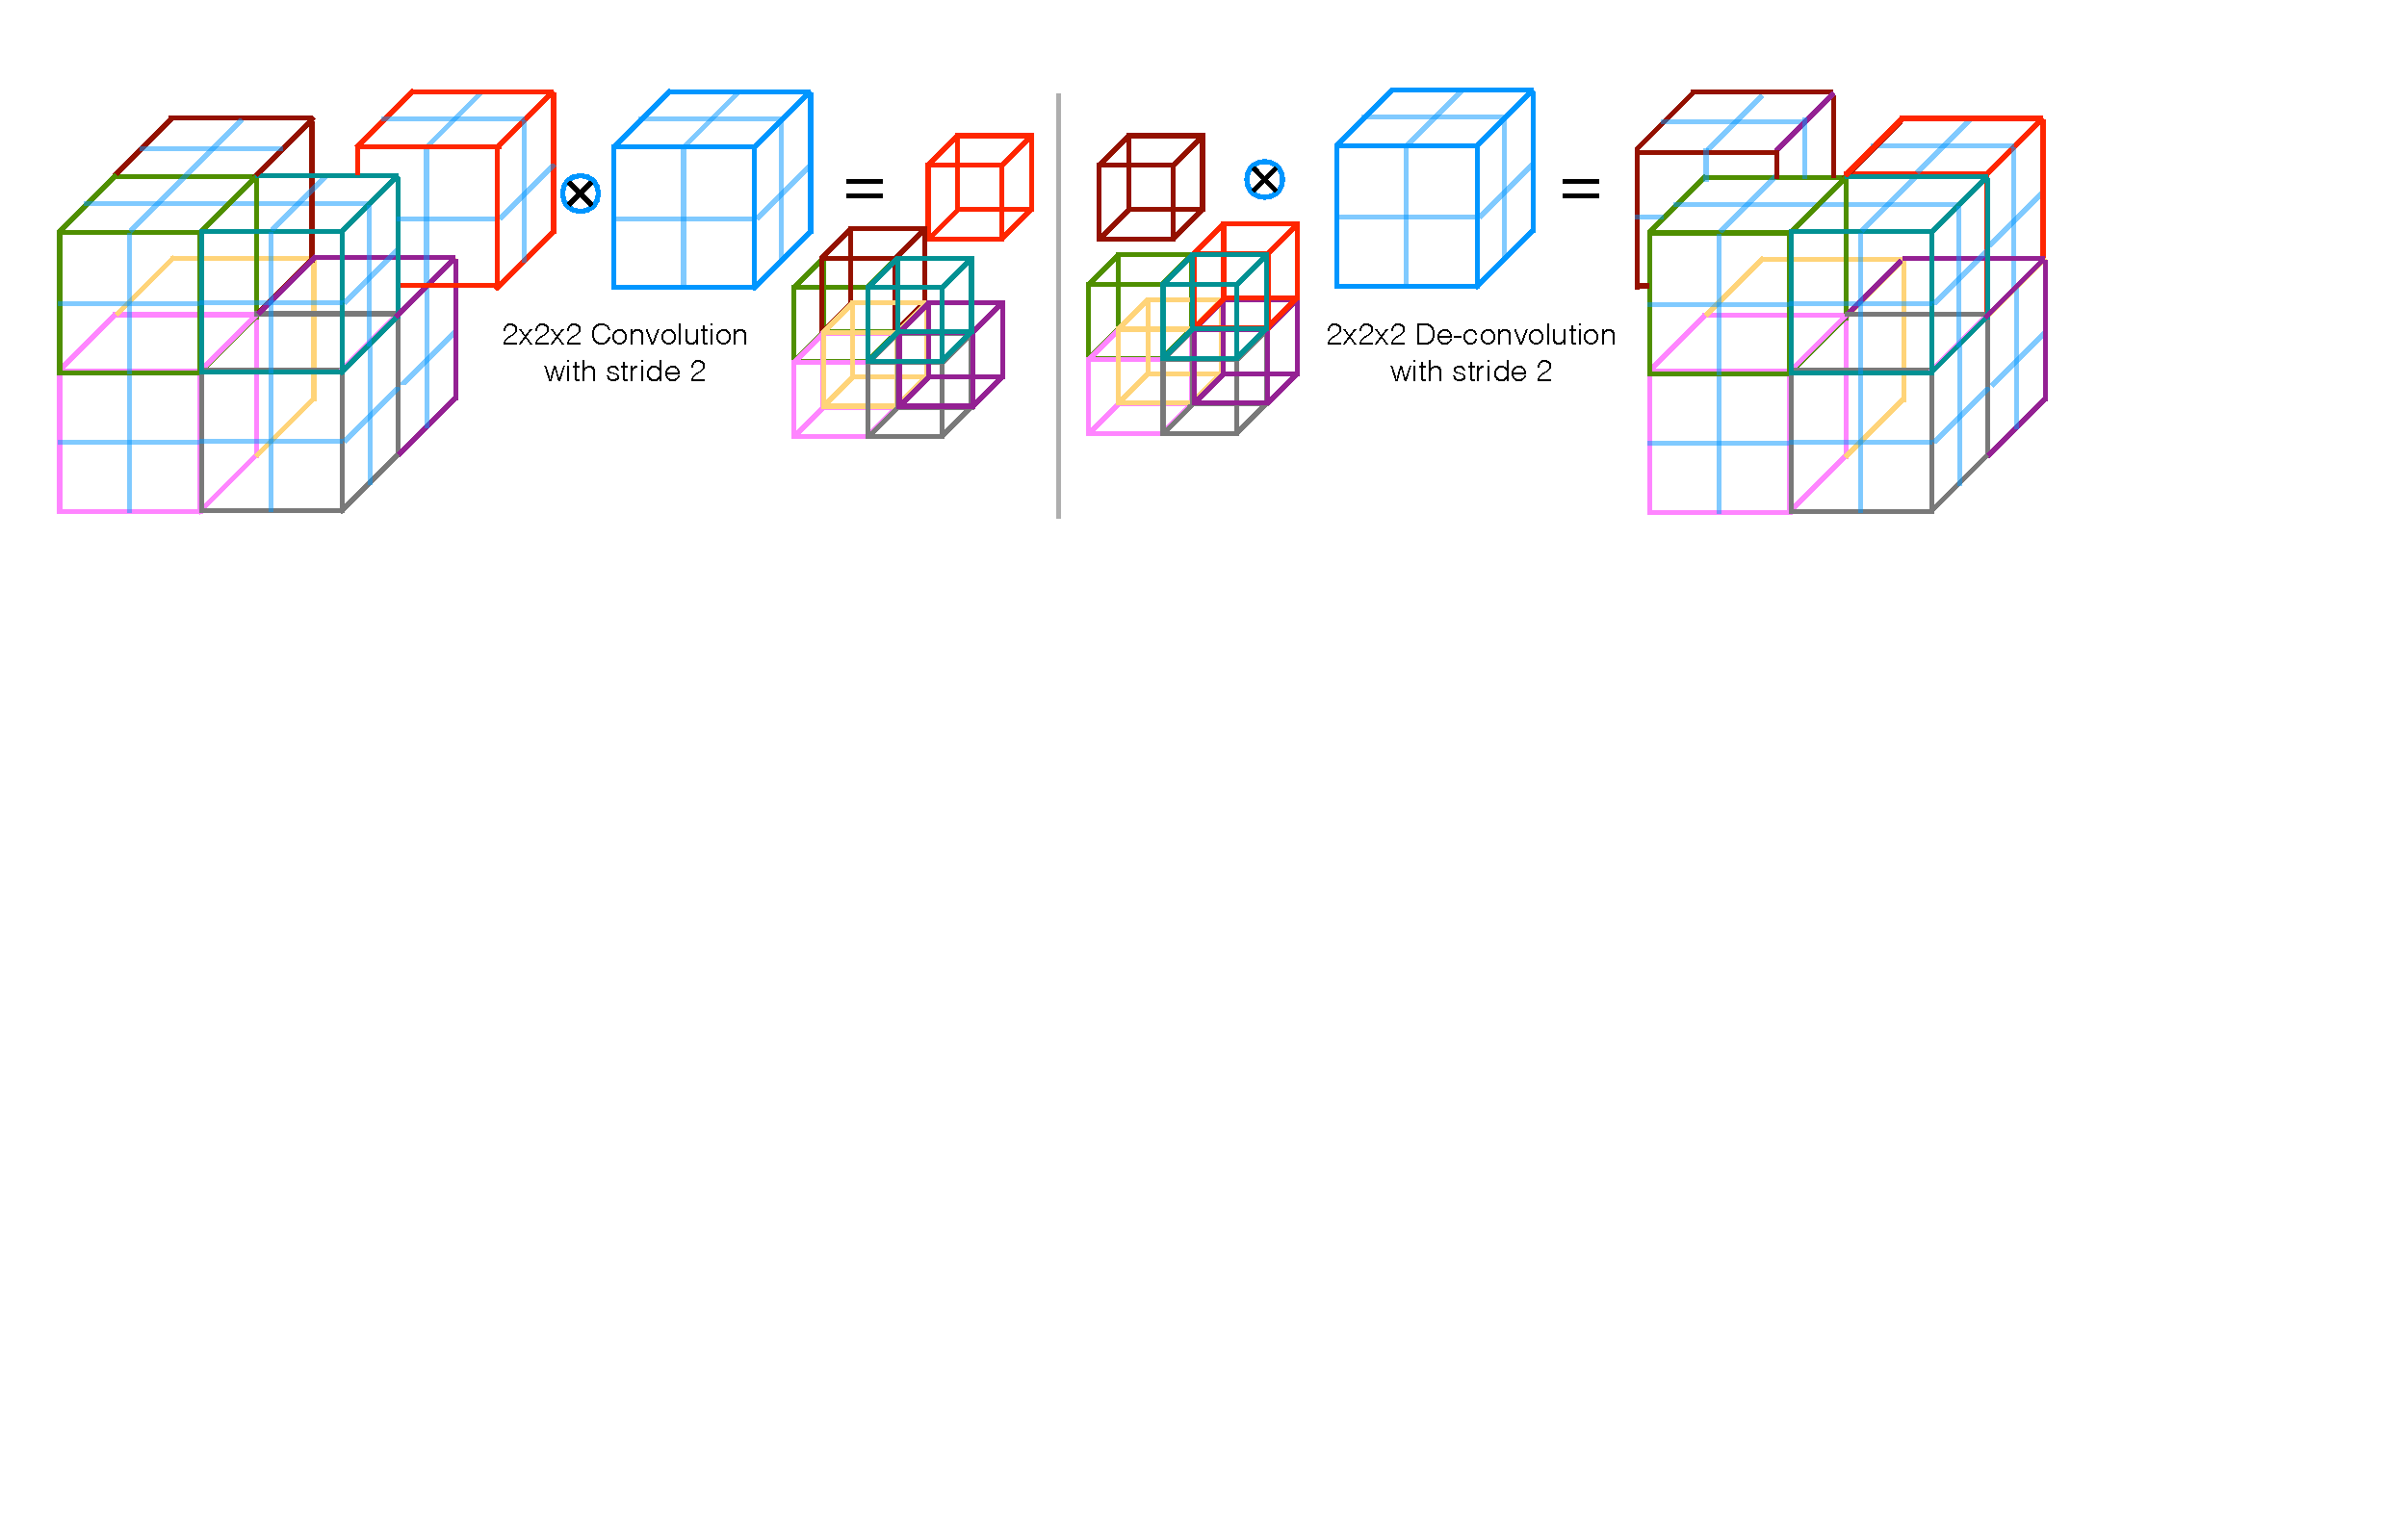
\includegraphics[scale=0.34]{updown.pdf} 	
\caption{Convolutions with appropriate stride can be used to reduce the size of the data. Conversely, de-convolutions increase the data size by projecting each input voxel to a bigger region through the kernel.} \label{fig:updown} 
\end{figure}

Similarly to \cite{ronneberger2015u}, we forward the features extracted from early stages of the left part of the CNN to the right part. This is schematically represented in Figure \ref{fig:VnetImage} by horizontal connections. In this way we gather fine grained detail that would be otherwise lost in the compression path and we improve the quality of the final contour prediction. We also observed that when these connections improve the convergence time of the model.

We report in Table \ref{table:receptiveFields} the receptive fields of each network layer, showing the fact that the innermost portion of our CNN already captures the content of the whole input volume. We believe that this characteristic is important during segmentation of poorly visible anatomy: the features computed in the deepest layer perceive the whole anatomy of interest at once, since they are computed from data having a spatial support much larger than the typical size of the anatomy we seek to delineate, and therefore impose global constraints.

\begin{table}
\begin{centering}
\protect\caption{Theoretical receptive field of the $3\times3\times3$ convolutional layers of the network.} 
\begin{tabular}{|c|c|c||c|c|c|}
\hline 
Layer & Input Size & Receptive Field & Layer & Input Size & Receptive Field\tabularnewline
\hline 
\hline 
L-Stage 1 & $128$ & $5\times5\times5$ & R-Stage 4 & 16 & $476\times476\times476$\tabularnewline
\hline 
L-Stage 2 & $64$ & $22\times22\times22$ & R-Stage 3 & 32 & $528\times528\times528$\tabularnewline
\hline 
L-Stage 3 & $32$ & $72\times72\times72$ & R-Stage 2 & 64 & $546\times546\times546$\tabularnewline
\hline 
L-Stage 4 & $16$ & $172\times172\times172$ & R-Stage 1 & 128 & $551\times551\times551$\tabularnewline
\hline 
L-Stage 5 & $8$ & $372\times372\times372$ & Output & 128 & \textbf{$551\times551\times551$}\tabularnewline
\hline 
\end{tabular} \label{table:receptiveFields}
\par\end{centering}
\end{table}

\section{Dice loss layer}
The network predictions, which consist of two volumes having the same resolution as the original input data, are processed through a soft-max layer which outputs the probability of each voxel to belong to foreground and to background. In medical volumes such as the ones we are processing in this work, it is not uncommon that the anatomy of interest occupies only a very small region of the scan. This often causes the learning process to get trapped in local minima of the loss function yielding a network whose predictions are strongly biased towards background. As a result the foreground region is often missing or only partially detected. Several previous approaches resorted to loss functions based on sample re-weighting where foreground regions are given more importance than background ones during learning. In this work we propose a novel objective function based on dice coefficient, which is a quantity ranging between $0$ and $1$ which we aim to maximise. The dice coefficient $D$ between two binary volumes can be written as
\[
D=\frac{2\sum_{i}^{N}p_{i}g_{i}}{\sum_{i}^{N}p_{i}^{2}+\sum_{i}^{N}g_{i}^{2}}
\]

where the sums run over the $N$ voxels, of the predicted binary segmentation volume $p_i\in{P}$ and the ground truth binary volume $g_i\in{G}$. This formulation of Dice can be differentiated yielding the gradient  
\[
\frac{\partial D}{\partial p_{j}}=2\left[\frac{g_{j}\left(\sum_{i}^{N}p_{i}^{2}+\sum_{i}^{N}g_{i}^{2}\right)-2p_{j}\left(\sum_{i}^{N}p_{i}g_{i}\right)}{\left(\sum_{i}^{N}p_{i}^{2}+\sum_{i}^{N}g_{i}^{2}\right)^{2}}\right]
\]
computed with respect to the $j$-th voxel of the prediction. Using this formulation we do not need to assign weights to samples of different classes to establish the right balance between foreground and background voxels, and we obtain results that we experimentally observed are much better than the ones computed through the same network trained optimising a multinomial logistic loss with sample re-weighting (Fig. \ref{fig:qualitativecomparison}). 

\subsection{Training}
Our CNN is trained end-to-end on a dataset of prostate scans in MRI. An example of the typical content of such volumes is shown in Figure \ref{fig:anatomies}. All the volumes processed by the network have fixed size of $128\times128\times64$ voxels and a spatial resolution of $1\times1\times1.5$ millimeters.

Annotated medical volumes are not easy to obtain due to the fact that one or more experts are required to manually trace a reliable ground truth annotation and that there is a cost associated with their acquisition. In this work we found necessary to augment the original training dataset in order to obtain robustness and increased precision on the test dataset. 

During every training iteration, we fed as input to the network randomly deformed versions of the training images by using a dense deformation field obtained through a $2\times2\times2$ grid of control-points and B-spline interpolation. This augmentation has been performed "on-the-fly", prior to each optimisation iteration, in order to alleviate the otherwise excessive storage requirements. Additionally we vary the intensity distribution of the data by adapting, using histogram matching, the intensity distributions of the training volumes used in each iteration, to the ones of other randomly chosen scans belonging to the dataset.

\subsection{Testing}
A Previously unseen MRI volume can be segmented by processing it in a feed-forward manner through the network. The output of the last convolutional layer, after soft-max, consists of a probability map for background and foreground. The voxels having higher probability ($>0.5$) to belong to the foreground than to the background are considered part of the anatomy.
